% This is samplepaper.tex, a sample chapter demonstrating the
% LLNCS macro package for Springer Computer Science proceedings;
% Version 2.21 of 2022/01/12
%
\documentclass[runningheads]{llncs}
%
\usepackage[svgnames]{xcolor}
\usepackage[T1]{fontenc}
% T1 fonts will be used to generate the final print and online PDFs,
% so please use T1 fonts in your manuscript whenever possible.
% Other font encondings may result in incorrect characters.
%
\usepackage{graphicx}
\graphicspath{{images/}} %configuring the graphicx package
% Used for displaying a sample figure. If possible, figure files should
% be included in EPS format.
%
% If you use the hyperref package, please uncomment the following two lines
% to display URLs in blue roman font according to Springer's eBook style:
%\usepackage{color}
%\renewcommand\UrlFont{\color{blue}\rmfamily}
%\urlstyle{rm}
%
\begin{document}
%
\title{Report on: Natural Software Revisited}
%
%\titlerunning{Abbreviated paper title}
% If the paper title is too long for the running head, you can set
% an abbreviated paper title here
%
\author{Zuxing Wu}
%
\authorrunning{Z. Wu}
% First names are abbreviated in the running head.
% If there are more than two authors, 'et al.' is used.
%
\institute{University of Adelaide, Adelaide, SA 5005, Australia\\
\email{a1816653@adelaide.edu.au}}
%
\maketitle              % typeset the header of the contribution
%
%
\section{Introduction}
\subsection{Motivation}
Language modelling is a widely used technique in Statistical Machine Translation (SMT) [26] and Natural Language Processing (NLP) [24]. After training a language model on a large corpus of code, it then shows that previously seen code has high naturalness, while unseen code has lower naturalness. To figure out what the ‘naturalness’ of software code means, whether it means repetitiveness and predictability, researchers need to conduct necessary preprocessing on code of different programming languages. Similar to NLP methods, different tasks require different preprocessing methods, e.g. tuning or cleaning. If someone wants to develop a tool for English grammar detection and improvement, stopwords such as ‘in, on, the, of, this’ should be kept. If extracting topics from articles is the goal, then stopwords could be deleted since they will introduce noise and make predictions less accurate. If aiming to spot syntax errors, then SyntaxTokens must be kept. On the contrary, if recommending possible code snippets is the goal, SyntaxTokens will reduce the prediction chances.

\subsection{Relevant Work}
\subsubsection{Research into language entropy\\}
There is a long history of language entropy measurement for understanding the redundancy of words. Shannon~\cite{ref_shannon1951} developed a method of statistical measures of English language entropy. After that, Gabel and Su~\cite{ref_chen2001} found code is highly redundant. Hindle et al.~\cite{ref_hindle2012}, following this path, verified that programs are very repetitive and predictable. Other works also examined that repetition happens at higher granularity [30], from package, and class to statement, line, and even word level. Repetition has also been studied in Android Apps [4, 29]. All of the research proves that code is repetitive and follows a predictable pattern.

\subsubsection{Research on code validation and checking\\}
Static analysis is often used for detecting code defects and faults. Recent works show it is common to use statistical features of languages for bugs detection and patches generating. Campbell et al.~\cite{ref_campbell2014} discover that n-gram language models are helpful in syntax error detection. Some researchers state bugs normally are less natural on having relatively high entropy~\cite{ref_jimenez2018}. Santos and Hindle~\cite{ref_santos2016} present that the cross-entropy of text split into n-grams in commit messages is an effective way of detecting bad commits that can cause build failure.

\subsubsection{Research on recommenders and autocompletion\\}
Most IDE tools provide the function of autocompletion that can suggest a next word, or snippets based on the structure of existing code. Researchers must have known code is repetitive before they work on the development of code prediction function. We can give appropriate guidance to coders during their activities by comparing the similarity rate of written code~\cite{ref_atkins1998}, commit marks~\cite{ref_chen2001}, besides API usages [33].  We can recommend relevant source code by using association rule mining on the CVS repository~\cite{ref_zimmermann2005}. Azad et al.~\cite{ref_azad2017} have been able to generate reliable change rule predictions from related Apps and the code snippets on StackOverflow. Sophisticated recommendations can be achieved by combining the history of code and the repetitiveness of programs to generate code components for coders. Buse and Weimer~\cite{ref_azad2017} succeed in generating automatic code recommendations from a large corpus of using-API code. Nguyen et al.~\cite{ref_nguyen2013} managed to recommend accurate snippets by using statistical language models. The following work of Nguyen and Nguyen~\cite{ref_nguyen2013} can create syntactically valid recommendations by adopting graph representations.

\subsubsection{Research on statistical translation\\}
Google Translate is a good example of translating English to code by copying the successful mechanism of Statistical Machine Translation in natural languages. SWIM~\cite{ref_raghothaman2016} can generate API sample snippets through a query corpus from Bing to align English and code. DeepAPI~\cite{ref_gu2016} trains recurrent neural networks on aligned source code comments with code for translating longer sequences of API calls. T2API~\cite{ref_nguyen2013,ref_nguyen2016} can generate a set of API calls as well as producing extensive graphs of common API usages by aligning English text with code from StackOverflow posts. By comparison, T2API can produce more complex usages by re-ordering API elements, while SWIM and DeepAPI only produce short and simplistic code sequences because of their left-to-right preprocessing of code.

\section{Summary \& Compare}
The research of this article mainly focuses on proving the repetitiveness and predictability of API usages, which obviously supports API recommendation approaches. It also shows graphs are a more appropriate representation of programming languages. They used a large corpus of 7 programming languages from GitHub.  Necessary and sufficient comparisons were made during the research process. Table~\ref{tab1} on the next page shows the proportions of tokens of each programming language.

\begin{table}
\centering
\caption{Corpus size in tokens. Table 1 of Rahman et al.\cite{0_ref_proc1}}\label{tab1}
\begin{tabular}{l | l | l | l}
    \hline
    {\bfseries Language} &  {\bfseries Files} & {\bfseries Total Tokens} & {\bfseries Unique Tokens}\\
    \hline
    \hline
    Java &  26938 & 24091076 & 388399 (1.61\%) \\
    \hline
    C\# &  23186 & 24217086 & 389800 (1.61\%) \\
    \hline
    C &  10932 & 25255417 & 938434 (3.72\%) \\
    \hline
    JavaScript &  10544 & 25157297 & 257606 (1.02\%) \\
    \hline
    Python &  15454 & 23198691 & 513728 (2.21\%) \\
    \hline
    Ruby &  60371 & 25896601 & 715157 (2.76\%)\\
    \hline
    Scala &  34242 & 23634250 & 333794 (1.41\%)\\
    \hline
\end{tabular}
\end{table}

The naturalness of source code stems from language-specific syntax, particularly separators and semicolons, which make up 44\% of all tokens in a Java corpus. Although code remains repetitive and predictable (to a lesser extent) even after removing punctuation and stopwords. They adopt Hindle et al.’s~\cite{ref_hindle2012} equation for calculating cross-entropy of a document D in a language model M:

\begin{equation}
    H(D, M) = -\frac{1}{n} \sum_{i=1}^{n} \log_2 P(t_i | t_{1}t_{2}...t_{i-1})
\end{equation}

Instead of developing the language model M from other documents and corpus, they divide a single corpus into 10 folds. Model is trained from 9 of the folds and H (D, M) is calculated with the remaining fold of D. By calculating the average value of all folds, we get the final SelfCrossEntropy. Lower SelfCrossEntropy means higher repetitiveness. As shown below in Figure~\ref{fig1}, scala is much less repetitive compared with C\#. 

\begin{figure}[h]
\centering
    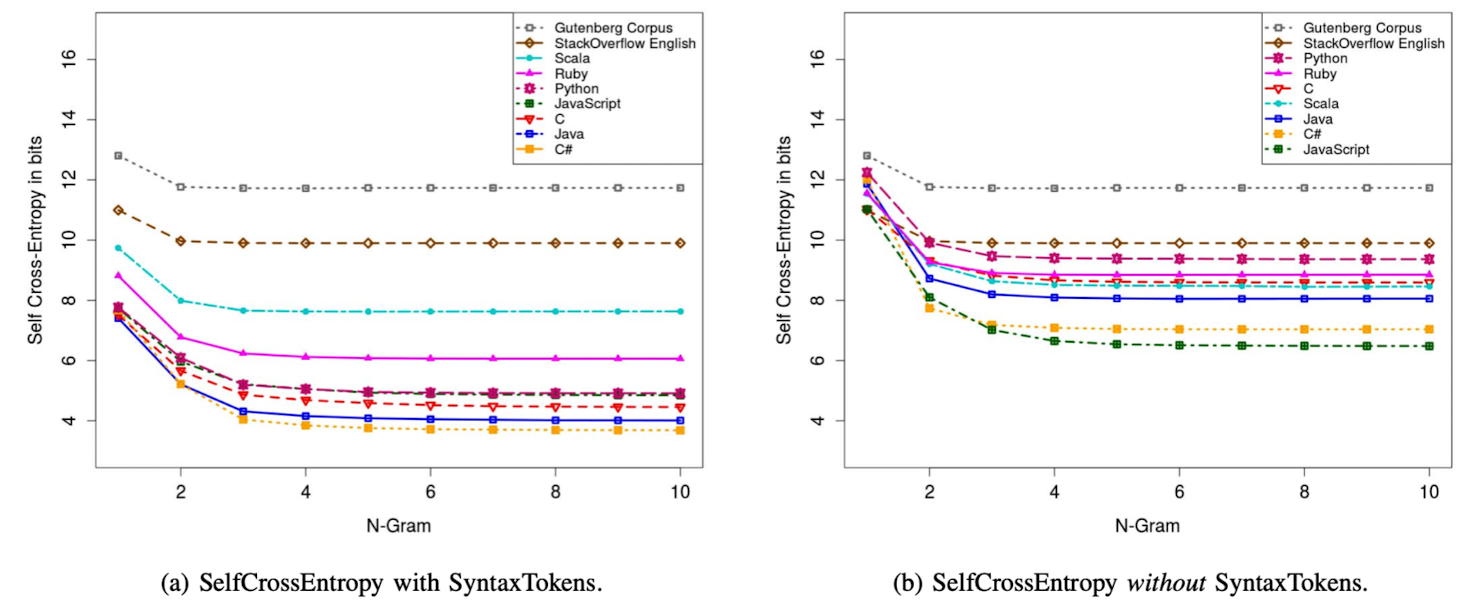
\includegraphics[width=\textwidth]{fig1}
    \caption{SelfCrossEntropy changes. Figure 2 of Rahman et al.\cite{0_ref_proc1}}\label{fig1}
\end{figure}

Programming languages become less repetitive when SyntaxTokens are removed. Technical discussions in English on StackOverflow exhibit a similar degree of repetition as code.
API code usages are highly repetitive because certain API calls, such as opening and closing files, are common across various programs and projects. This Figure~\ref{fig2} suggests 
that raw Java code, which includes SyntaxTokens, is more repetitive than Java API 
usages, likely due to the frequent application of syntax rules.

\begin{figure}[h]
\centering
    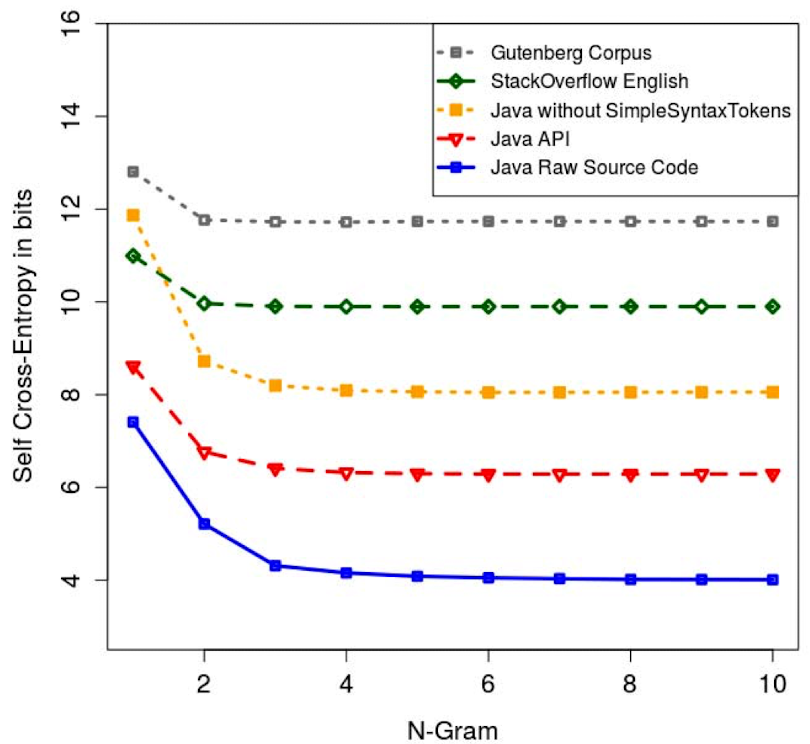
\includegraphics[width=\textwidth]{fig2}
    \caption{Comparison of Java SelfCrossEntropy. Figure 3 of Rahman et al.\cite{0_ref_proc1}}\label{fig2}
\end{figure}

Applications can leverage this feature to recommend sophisticated API call sequences using reliable statistical models. Although n-gram models were developed for natural languages, they are not well-suited for representing code, which is typically structured as an Abstract Syntax Tree (AST). AST contains control and data flow. By comparison, statistical graph representations can extract higher-level patterns than n-grams. It can even capture complex coding patterns. For example, the structure of iteration through a HashMap, as the Figure~\ref{fig3} below shows.

\begin{figure}[h]
\centering
    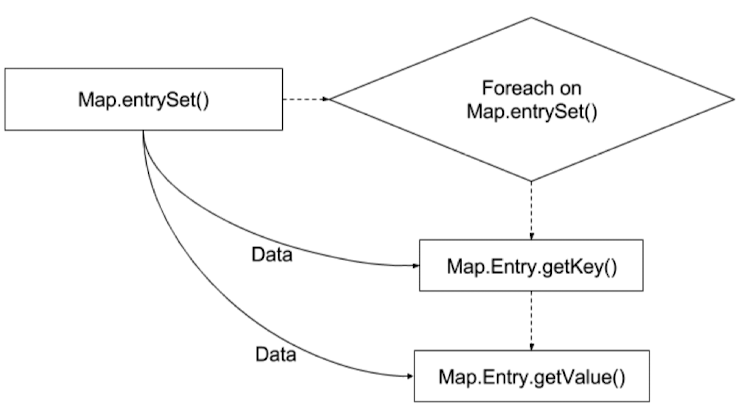
\includegraphics[width=\textwidth]{fig3}
    \caption{A GROUM representing iteration on a HashMap. Figure 5 of Rahman et al.\cite{0_ref_proc1}}\label{fig3}
\end{figure}

\section{Future Suggestions}
The outcomes of this research paper are obviously correct and convincing. However, some flaws exist in their recommended graph model. For example, GROUM can not generate graph presentations successfully if one node is missing. Future works should try to solve this problem to make it more robust. Secondly, the computational expense of identifying isomorphic or similar graphs is relatively higher, but fewer nodes are needed to represent the same block of code compared to sequential n-grams. Higher n-node graphs exhibit similar degrees of repetition as 3-node and 4-node graphs. SelfCrossEntropy has the limitation of being impractical to calculate all possible combinations of the next token due to its complexity, which is O(tn), where t represents the number of unique tokens and n represents the total number of tokens in the corpus. In practice, for each chosen language, there are over 300,000 unique tokens and 20 million total tokens.
To summarise, the GROUM is not reliable enough now. It needs some improvements in the future. The model is a bit time-consuming even though it works as a good approximation of entropy. Future research can focus on how to optimize the efficiency of the calculation or simplify the process.

\section{Critical Review}

\subsection{Strengths}
They created sufficient evidence that proves that source code is repetitive and predictable using projects of 7 programming languages (i.e. Java, C\#, C, JavaScript, Python, Ruby, Scala) picked from GitHub. 134 open-source projects are included in the code corpus. For comparison, they also selected two kinds of English corpus: Gutenberg corpus, and StackOverflow posts. The contribution of SyntaxTokens to repetition was confirmed by the comparison of SelfCrossEntropy between the original code and the code without SyntaxTokens. Furthermore, API usage is also a factor that makes the code repetitive. By comparing the repetitiveness of n-grams and graph representations of code, it is evident that graph representations are more repetitive than sequential ones. Consequently, they are more suitable for code recommendation tasks because they can capture non-sequential and complex relationships within the code.

\subsection{Weaknesses}
There are not many bad or not-good-enough things about this research. What it states are just some plain truths that are basically the same as our guess. If I have to say something not good, it’s this research did not surprise me. I want to learn something and get some suggestions about how students can avoid the high similarity rate of their code if they use code recommendation or autocompletion applications. This research only says that a graph is more appropriate than an n-gram model in code prediction.

\subsection{My Method}
No extra method is needed for this paper. They have done very good research on this area even though the results are not very surprising but at least is inspiring. They offered their GitHub repository containing scripts and output data for future researchers to reproduce and check the results, or reuse for new relevant research.

% ---- Bibliography ----
%
% BibTeX users should specify bibliography style 'splncs04'.
% References will then be sorted and formatted in the correct style.
%
% \bibliographystyle{agsm}
\bibliographystyle{splncs04}
% \bibliography{mybibliography}
%
\newpage
\begin{thebibliography}{8}
    \bibitem{0_ref_proc1}
    Rahman, M., Palani, D., Rigby, P.C.: Natural Software Revisited. In: 2019 IEEE/ACM 41st International Conference on Software Engineering (ICSE), pp. 37--48. IEEE (2019)

    \bibitem{ref_koehn2009}
    Koehn, P.: Statistical machine translation. Cambridge University Press (2009)
    
    \bibitem{ref_jones1994}
    Jones, K.S.: Natural language processing: a historical review. In: Current issues in computational linguistics: in honour of Don Walker, pp. 3--16. Springer (1994)
    
    \bibitem{ref_shannon1951}
    Shannon, C.E.: Prediction and entropy of printed English. Bell Labs Technical Journal \textbf{30}(1), 50--64 (1951)
    
    \bibitem{ref_gabel2010}
    Gabel, M., Su, Z.: A study of the uniqueness of source code. In: Proceedings of the Eighteenth ACM SIGSOFT International Symposium on Foundations of Software Engineering, FSE ’10, pp. 147--156. ACM, New York, NY, USA (2010)
    
    \bibitem{ref_hindle2012}
    Hindle, A., Barr, E.T., Su, Z., Gabel, M., Devanbu, P.: On the naturalness of software. In: Proceedings of the 34th International Conference on Software Engineering, ICSE ’12, pp. 837--847. IEEE Press, Piscataway, NJ, USA (2012)
    
    \bibitem{ref_santos2016}
    Santos, E.A., Hindle, A.: Judging a commit by its cover: Correlating commit message entropy with build status on travis-ci. In: Proceedings of the 13th International Conference on Mining Software Repositories, MSR ’16, pp. 504--507. ACM, New York, NY, USA (2016)
    
    \bibitem{ref_atkins1998}
    Atkins, D.L.: Version sensitive editing: Change history as a programming tool. In: Magnusson, B. (ed.) SCM, Lecture Notes in Computer Science, vol. 1439, pp. 146--157. Springer (1998)
    
    \bibitem{ref_chen2001}
    Chen, A., Chou, E., Wong, J., Yao, A.Y., Zhang, Q., Zhang, S., Michail, A.: Cvssearch: Searching through source code using cvs comments. In: ICSM, pp. 364--. (2001)
    
    \bibitem{ref_michail1999}
    Michail, A.: Data mining library reuse patterns in user-selected applications. In: Proceedings of the 14th IEEE International Conference on Automated Software Engineering, ASE ’99, pp. 24--. IEEE Computer Society, Washington, DC, USA (1999)
    
    \bibitem{ref_zhang2010}
    Zhang, Y.F., Zhang, Q.F., Yu, R.H.: Markov property of markov chains and its test. In: 2010 International Conference on Machine Learning and Cybernetics, vol. 4, pp. 1864--1867. (July 2010)
    
    \bibitem{ref_buse2012}
    Buse, R.P.L., Weimer, W.: Synthesizing API usage examples. In: Proceedings of the 20th International Conference on Software Engineering, pp. 782--792. (2012)
    
    \bibitem{ref_nguyen2013}
    Nguyen, T.T., Nguyen, A.T., Nguyen, H.A., Nguyen, T.N.: A statistical semantic language model for source code. In: Proceedings of the 2013 9th Joint Meeting on Foundations of Software Engineering, ESEC/FSE 2013, pp. 532--542. ACM, New York, NY, USA (2013)
    
    \bibitem{ref_lin2017}
    Lin, B., Ponzanelli, L., Mocci, A., Bavota, G., Lanza, M.: On the uniqueness of code redundancies. In: 2017 IEEE/ACM 25th International Conference on Program Comprehension (ICPC), pp. 121--131. (May 2017)
    
    \bibitem{ref_azad2017}
    Azad, S., Rigby, P.C., Guerrouj, L.: Generating API Call Rules from Version History and Stack Overflow Posts. ACM Trans. Softw. Eng. Methodol., 25(4), 29:1--29:22. (Jan. 2017)
    
    \bibitem{ref_lamba2015}
    Lamba, Y., Khattar, M., Sureka, A.: Pravaaha: Mining Android applications for discovering API call usage patterns and trends. In: Proceedings of the 8th India Software Engineering Conference, pp. 10--19. ACM (2015)
    
    \bibitem{ref_campbell2014}
    Campbell, J.C., Hindle, A., Amaral, J.N.: Syntax errors just aren’t natural: Improving error reporting with language models. In: Proceedings of the 11th Working Conference on Mining Software Repositories, MSR 2014, pp. 252--261. ACM, New York, NY, USA (2014)
    
    \bibitem{ref_jimenez2018}
    Jimenez, M., Maxime, C., Le Traon, Y., Papadakis, M.: On the impact of tokenizer and parameters on n-gram based code analysis. In: 2018 IEEE International Conference on Software Maintenance and Evolution (ICSME), pp. 437--448. (Sep. 2018)
    
    \bibitem{ref_nguyen2018}
    Nguyen, T., Rigby, P.C., Nguyen, A.T., Dharani, M., Karanfil, P., Nguyen, T.N.: Statistical Translation of English Texts to API Code Templates. In: Proceedings of the 2018 IEEE International Conference on Software Maintenance and Evolution, ICSME ’18. IEEE Computer Society (2018)
    
    \bibitem{ref_raghothaman2016}
    Raghothaman, M., Wei, Y., Hamadi, Y.: Swim: Synthesizing what i mean: Code search and idiomatic snippet synthesis. In: Proceedings of the 38th International Conference on Software Engineering, ICSE ’16, pp. 357--367. ACM, New York, NY, USA (2016)
    
    \bibitem{ref_gu2016}
    Gu, X., Zhang, H., Zhang, D., Kim, S.: Deep API learning. In: Proceedings of the 2016 24th ACM SIGSOFT International Symposium on Foundations of Software Engineering, FSE 2016, pp. 631--642. ACM (2016)
    
    \bibitem{ref_nguyen2016}
    Nguyen, T., Rigby, P.C., Nguyen, A.T., Karanfil, M., Nguyen, T.N.: T2API: Synthesizing API Code Usage Templates from English Texts with Statistical Translation. In: Proceedings of the 2016 24th ACM SIGSOFT International Symposium on Foundations of Software Engineering (Formal Demostration Track), FSE 2016, pp. 1013--1017. ACM (2016)
    
    \bibitem{ref_hindle2012}
    Hindle, A., Barr, E.T., Su, Z., Gabel, M., Devanbu, P.: On the naturalness of software. In: Proceedings of the 34th International Conference on Software Engineering, ICSE ’12, pp. 837--847. IEEE Press, Piscataway, NJ, USA (2012)

    \bibitem{ref_zimmermann2005}
    Zimmermann, T., Weißgerber, P., Diehl, S., Zeller, A.: Mining version histories to guide software changes. IEEE Transactions on Software Engineering, 31(6), pp. 429--445. (June 2005)
% %%%%%%%%%%%%%%%%%%%%%%%%%%%%%%%%%%%%%%%%%%%%%%%%%%%%%%%%%%%%%%%%%%%%%%%%%%%%%
% \bibitem{ref_article}
% Author, F.: Article title. Journal \textbf{2}(5), 99--110 (2016)

% \bibitem{ref_lncs1}
% Author, F., Author, S.: Title of a proceedings paper. In: Editor,
% F., Editor, S. (eds.) CONFERENCE 2016, LNCS, vol. 9999, pp. 1--13.
% Springer, Heidelberg (2016). \doi{10.10007/1234567890}

% \bibitem{ref_book1}
% Author, F., Author, S., Author, T.: Book title. 2nd edn. Publisher,
% Location (1999)

% \bibitem{ref_proc}
% Author, A.-B.: Contribution title. In: 9th International Proceedings
% on Proceedings, pp. 1--2. Publisher, Location (2010)

% \bibitem{ref_url1}
% LNCS Homepage, \url{http://www.springer.com/lncs}, last accessed 2023/10/25
\end{thebibliography}
\end{document}
